\documentclass{beamer}
\usepackage[english,russian]{babel}
\usepackage[utf8]{inputenc}
\usepackage{amsmath}
\usepackage{hyperref}
\usetheme{Warsaw}
\usepackage{listings}
\usepackage{xcolor}
\usepackage{tikz}
\usetikzlibrary{graphs}
\usepackage{algpseudocode}

\lstset{
    frame=tb,
    tabsize=4,
    showstringspaces=false,
    numbers=left,
    commentstyle=\color{green},
    keywordstyle=\color{blue},
    stringstyle=\color{red},
    emph={baz},
    emphstyle=\textbf
}

\begin{document}

\title{SAT/SMT solvers\newline  8. Quantified Formulas}
\author{Roman Kholin}
\institute{Lomonosov Moscow State University}
\date{Moscow, 2023}

\begin{frame}
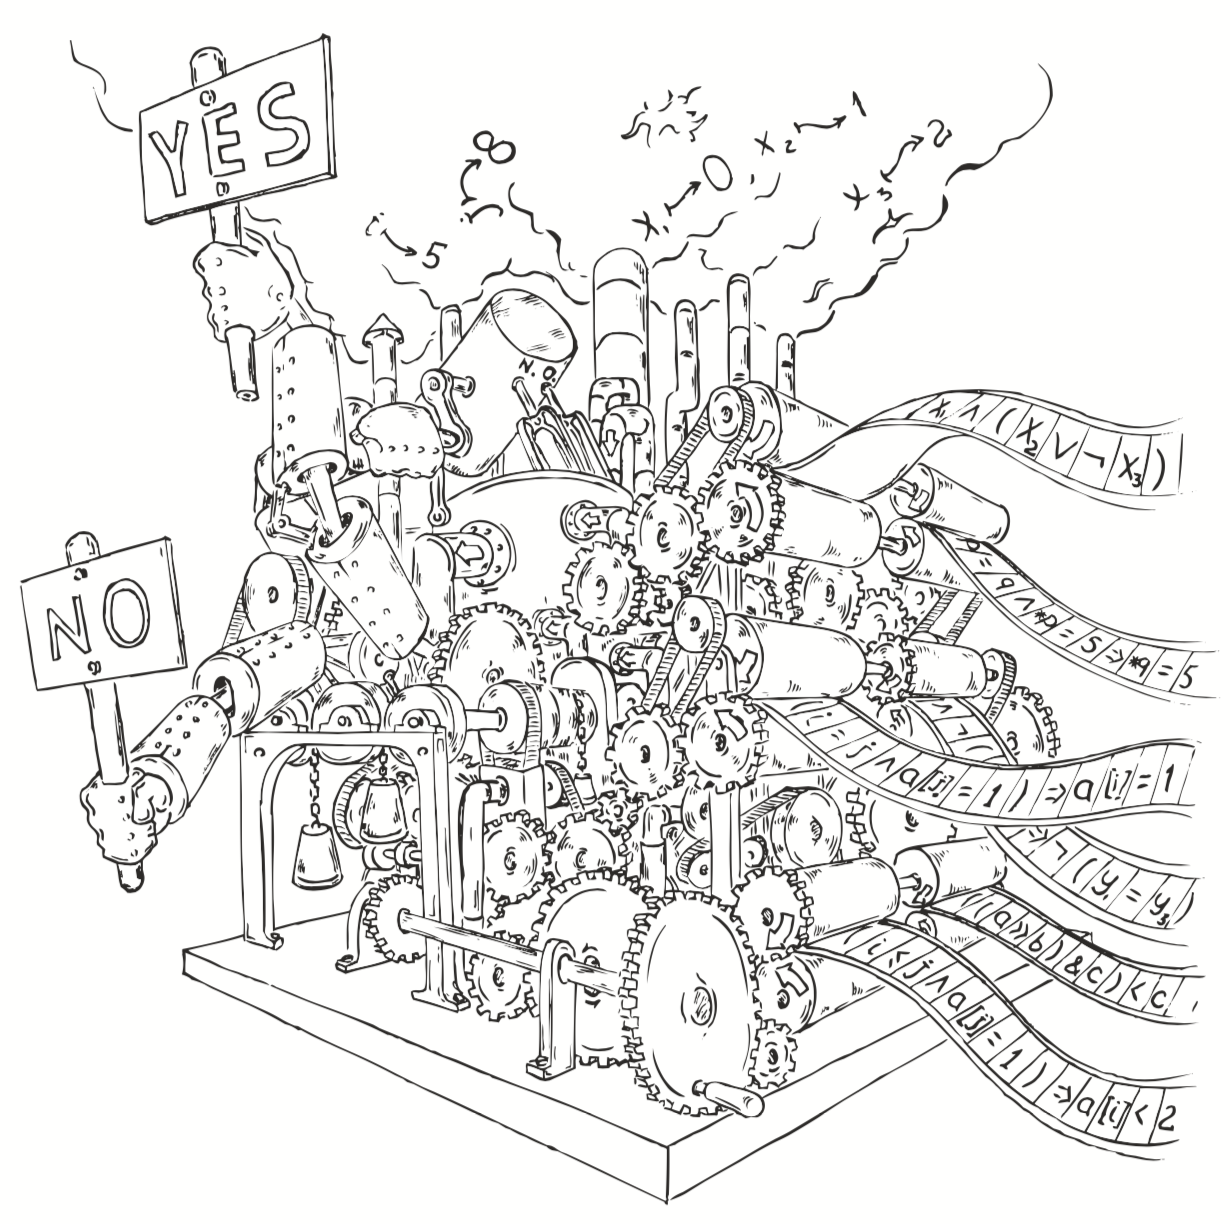
\includegraphics[scale=0.5]{../decision-procedure.png}
\end{frame}

\frame{\titlepage}

\begin{frame}{Definitions}
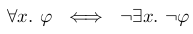
\includegraphics[scale=0.5]{all_and_exist.png}\newline
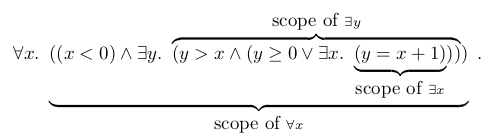
\includegraphics[scale=0.5]{scope.png}\newline
\begin{block}{}
\begin{itemize}
\item A variable is called free in a given formula if at least one of its occurrences is not bound by any quantifier
\item A formula Q is called a sentence (or closed) if none of its variables are free
\end{itemize}
\end{block}
\end{frame}

\begin{frame}{Syntax}
QBF:\newline
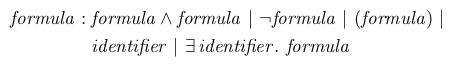
\includegraphics[scale=0.5]{qbf.png}\newline
Complexity - PSPACE\newline
QDLA:\newline
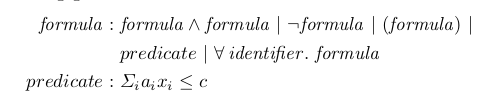
\includegraphics[scale=0.5]{qdla.png}\newline
\end{frame}

\begin{frame}{Definitions}
\begin{block}{Prenex normal form}
\begin{itemize}
\item A formula is said to be in prenex normal form (PNF) if it is in the form $Q[n]V[n]\dots Q[1]V[1].<quantifier-free formula>$, where $Q[i]$ - quantor, $V[i]$ - variable
\item For every quantified formula Q there exists a formula Q' in prenex normal form such that Q is valid if and only if Q' is valid
\end{itemize}
\end{block}
\end{frame}

\begin{frame}
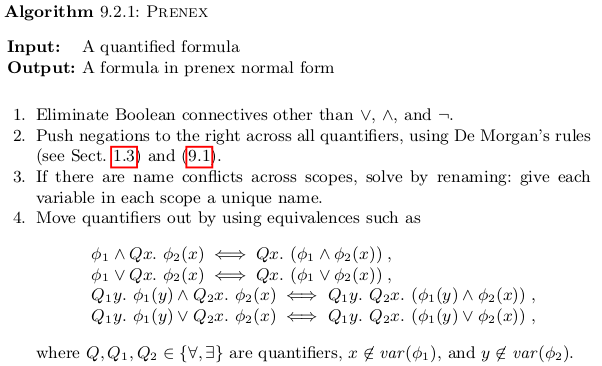
\includegraphics[scale=0.5]{prenex.png}\newline
\end{frame}

\begin{frame}{Example}
$\lnot\exists x.\lnot(\exists y.((y\implies x)\wedge(\lnot x\vee y))\wedge\lnot\forall y.((y\wedge x)\vee(\lnot x\wedge\lnot y)))$\newline
\end{frame}

\begin{frame}{Example}
$\lnot\exists x.\lnot(\exists y.((y\implies x)\wedge(\lnot x\vee y))\wedge\lnot\forall y.((y\wedge x)\vee(\lnot x\wedge\lnot y)))$\newline
$\forall x.(\exists y.((\lnot y\vee x)\wedge(\lnot x\wedge y)) \wedge\exists y.((\lnot y \vee\lnot x)\wedge(x\vee y)))$\newline
\end{frame}

\begin{frame}{Example}
$\lnot\exists x.\lnot(\exists y.((y\implies x)\wedge(\lnot x\vee y))\wedge\lnot\forall y.((y\wedge x)\vee(\lnot x\wedge\lnot y)))$\newline
$\forall x.(\exists y.((\lnot y\vee x)\wedge(\lnot x\wedge y))\wedge\exists y.((\lnot y \vee\lnot x)\wedge(x\vee y)))$\newline
$\forall x.(\exists y_1.((\lnot y_1\vee x)\wedge(\lnot x\wedge y_1))\wedge\exists y_2.((\lnot y_2 \vee\lnot x)\wedge(x\vee y_2)))$\newline
\end{frame}

\begin{frame}{Example}
$\lnot\exists x.\lnot(\exists y.((y\implies x)\wedge(\lnot x\vee y))\wedge\lnot\forall y.((y\wedge x)\vee(\lnot x\wedge\lnot y)))$\newline
$\forall x.(\exists y.((\lnot y\vee x)\wedge(\lnot x\wedge y))\wedge\exists y.((\lnot y \vee\lnot x)\wedge(x\vee y)))$\newline
$\forall x.(\exists y_1.((\lnot y_1\vee x)\wedge(\lnot x\wedge y_1))\wedge\exists y_2.((\lnot y_2\vee\lnot x)\wedge(x\vee y_2)))$\newline
$\forall x.\exists y_1 .\exists y_2 .(\lnot y_1 \vee x)\wedge(\lnot x \vee y_1) \wedge (\lnot y_2\vee\lnot x) \wedge(x\vee y_2).$\newline
\end{frame}

\begin{frame}{Projection}
Projection of $Q[n]V[n]\dots Q[2]V[2].\exists x.\phi$\newline
is $Q[n]V[n]\dots Q[2]V[2].\phi$\newline
\end{frame}

\begin{frame}
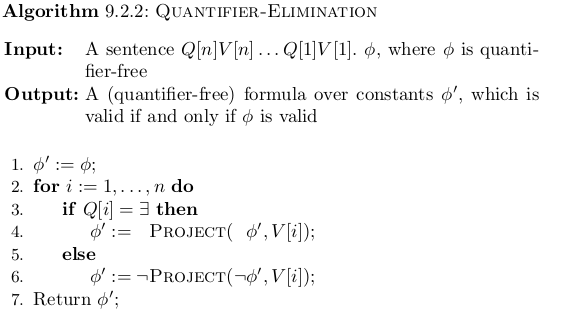
\includegraphics[scale=0.5]{quantifier-elimination.png}\newline
\end{frame}

\begin{frame}{Quantifier elimination for Quantified Boolean Formulas}
$\exists y.\exists z.\forall x.(y\vee x)\wedge(z\vee\lnot x) \wedge (y \vee \lnot z \vee \lnot x) \wedge (\lnot y \vee z)$\newline
$\exists y.\exists z.(y)\wedge(z) \wedge (y \vee \lnot z\vee) \wedge (\lnot y \vee z)$\newline
\end{frame}

\begin{frame}{Quantifier elimination for Quantified Boolean Formulas}
$\exists y.\exists z.\forall x.(y\vee x)\wedge(z\vee\lnot x) \wedge (y \vee \lnot z \vee \lnot x) \wedge (\lnot y \vee z)$\newline
$\exists y.\exists z.(y)\wedge(z) \wedge (y \vee \lnot z\vee) \wedge (\lnot y \vee z)$\newline
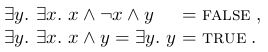
\includegraphics[scale=0.5]{elem_qbf1.png}\newline
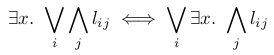
\includegraphics[scale=0.5]{elem_qbf2.png}\newline
\end{frame}

\begin{frame}{Quantifier elimination for Quantified Boolean Formulas}
$\exists y.\exists z.\forall x.(y\vee x)\wedge(z\vee\lnot x) \wedge (y \vee \lnot z \vee \lnot x) \wedge (\lnot y \vee z)$\newline
$\exists y.\exists z.(y)\wedge(z) \wedge (y \vee \lnot z\vee) \wedge (\lnot y \vee z)$\newline
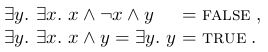
\includegraphics[scale=0.5]{elem_qbf1.png}\newline
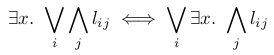
\includegraphics[scale=0.5]{elem_qbf2.png}\newline
$\exists y.\exists z.\exists x.(y\vee x)\wedge(z\vee\lnot x) \wedge (y \vee \lnot z \vee \lnot x) \wedge (\lnot y \vee z)$\newline
$\exists y.\exists z.(y\vee z)\wedge (y \vee \lnot z) \wedge (\lnot y \vee z)$\newline
\end{frame}

\begin{frame}{Quantifier elimination for Quantified Boolean Formulas}
$\exists y.\exists z.\forall x.(y\vee x)\wedge(z\vee\lnot x) \wedge (y \vee \lnot z \vee \lnot x) \wedge (\lnot y \vee z)$\newline
$\exists y.\exists z.(y)\wedge(z) \wedge (y \vee \lnot z\vee) \wedge (\lnot y \vee z)$\newline
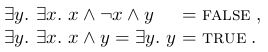
\includegraphics[scale=0.5]{elem_qbf1.png}\newline
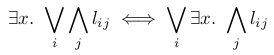
\includegraphics[scale=0.5]{elem_qbf2.png}\newline
$\exists y.\exists z.\exists x.(y\vee x)\wedge(z\vee\lnot x) \wedge (y \vee \lnot z \vee \lnot x) \wedge (\lnot y \vee z)$\newline
$\exists y.\exists z.(y\vee z)\wedge (y \vee \lnot z) \wedge (\lnot y \vee z)$\newline
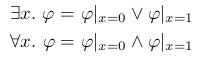
\includegraphics[scale=0.5]{expansion_based.png}
\end{frame}

\begin{frame}{Search-Based Algorithms for Quantified Boolean Formulas}
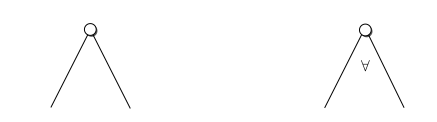
\includegraphics[scale=0.5]{cdcl1.png}
\end{frame}

\begin{frame}{Search-Based Algorithms for Quantified Boolean Formulas}
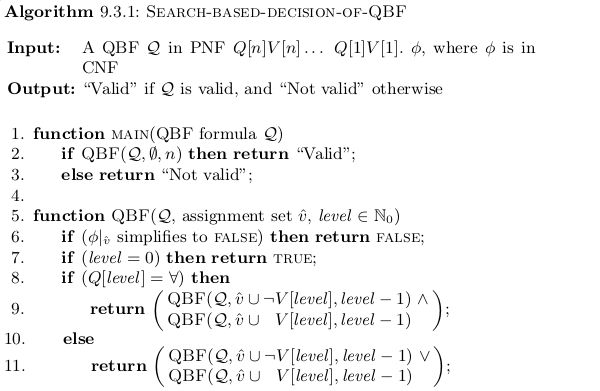
\includegraphics[scale=0.5]{cdcl2.png}
\end{frame}

\begin{frame}{Skolemization}
\begin{block}{Skolem normal form}
A formula is in Skolem normal form if it is in prenex normal form and has only universal quantifiers.
\end{block}
\begin{block}{Skolemization}
Let $\psi = \exists x$. $P$ be a subformula in $\varphi$. Let $y_1, \dots, y_n$ be universally quantified variables such that $\psi$ is
in their scope.
\begin{enumerate}
\item Remove the quantifier $\exists x$ from $\psi$
\item Replace occurrences of $x$ in $P$ with $f_x(y_1, \dots, y_n)$, where $f_x$ is a new function symbol. It is sufficient to include
those $y$ variables that are actually used in $P$. If $n = 0$, then replace x with a new constant $c_x$
\end{enumerate}
\end{block}
$\forall y_1.\forall y_2.f(y_1, y_2) \wedge \exists x.(f(x, y_2) \wedge x < 0)$\newline
\end{frame}

\begin{frame}{Skolemization}
\begin{block}{Skolem normal form}
A formula is in Skolem normal form if it is in prenex normal form and has only universal quantifiers.
\end{block}
\begin{block}{Skolemization}
Let $\psi = \exists x$. $P$ be a subformula in $\varphi$. Let $y_1, \dots, y_n$ be universally quantified variables such that $\psi$ is
in their scope.
\begin{enumerate}
\item Remove the quantifier $\exists x$ from $\psi$
\item Replace occurrences of $x$ in $P$ with $f_x(y_1, \dots, y_n)$, where $f_x$ is a new function symbol. It is sufficient to include
those $y$ variables that are actually used in $P$. If $n = 0$, then replace x with a new constant $c_x$
\end{enumerate}
\end{block}
$\forall y_1.\forall y_2.f(y_1, y_2) \wedge \exists x.(f(x, y_2) \wedge x < 0)$\newline
$\forall y_1.\forall y_2.f(y_1, y_2) \wedge (f(f_x(y_1, y_2), y_2) \wedge f_x(y_1, y_2) < 0)$\newline
\end{frame}

\begin{frame}{Instantiation}
A typical scenario: to prove the validity of a ground formula $G$ based on sentences that represent axioms.\newline
To prove $G$ we can try to $instantiate$ the universally quantified variables in order to reach a contradiction with $\lnot G$.
\end{frame}

\begin{frame}{Instantiation}
A typical scenario: to prove the validity of a ground formula $G$ based on sentences that represent axioms.\newline
To prove $G$ we can try to $instantiate$ the universally quantified variables in order to reach a contradiction with $\lnot G$.
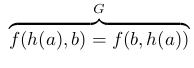
\includegraphics[scale=0.5]{ground.png}\newline
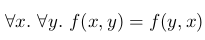
\includegraphics[scale=0.5]{axiom.png}\newline
\end{frame}

\begin{frame}{Instantiation}
A typical scenario: to prove the validity of a ground formula $G$ based on sentences that represent axioms.\newline
To prove $G$ we can try to $instantiate$ the universally quantified variables in order to reach a contradiction with $\lnot G$.
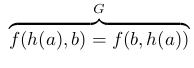
\includegraphics[scale=0.5]{ground.png}\newline
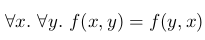
\includegraphics[scale=0.5]{axiom.png}\newline
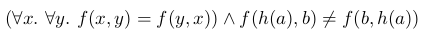
\includegraphics[scale=0.5]{toproof.png}\newline
\end{frame}

\begin{frame}{Instantiation}
A typical scenario: to prove the validity of a ground formula $G$ based on sentences that represent axioms.\newline
To prove $G$ we can try to $instantiate$ the universally quantified variables in order to reach a contradiction with $\lnot G$.
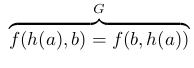
\includegraphics[scale=0.5]{ground.png}\newline
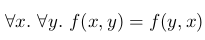
\includegraphics[scale=0.5]{axiom.png}\newline
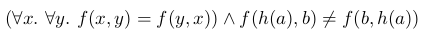
\includegraphics[scale=0.5]{toproof.png}\newline
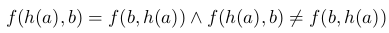
\includegraphics[scale=0.5]{instantiation.png}\newline
\end{frame}

\begin{frame}{Simple strategy}
Let $(\forall\overline{x}.\psi) \wedge G$ - formula that we attempt to prove to be unsatisfiable\newline
$Triggers$ - subterms in $\psi$ that contain references to all the variables in $\overline{x}$\newline
\begin{itemize}
\item For each quantified formula of the form $(\forall\overline{x}.\psi)$, identify all triggers
\item Try to match each trigger tr to an existing ground term $gr$ in $G$.
\item Given a substitution $\overline{s}$, assign $G := G \wedge \psi[\overline{x}\leftarrow\overline{s}]$ and check the satisfiability of
$G$
\end{itemize}
\end{frame}

\begin{frame}{Simple strategy}
Let $(\forall\overline{x}.\psi) \wedge G$ - formula that we attempt to prove to be unsatisfiable\newline
$Triggers$ - subterms in $\psi$ that contain references to all the variables in $\overline{x}$\newline
\begin{itemize}
\item For each quantified formula of the form $(\forall\overline{x}.\psi)$, identify all triggers
\item Try to match each trigger tr to an existing ground term $gr$ in $G$.
\item Given a substitution $\overline{s}$, assign $G := G \wedge \psi[\overline{x}\leftarrow\overline{s}]$ and check the satisfiability of
$G$
\end{itemize}
$G := (b = c \implies f(h(a), g(c)) = f(g(b), h(a)))$\newline
$\forall x.\forall y.f(x, y) = f(y, x)$\newline
\end{frame}

\begin{frame}{Simple strategy}
Let $(\forall\overline{x}.\psi) \wedge G$ - formula that we attempt to prove to be unsatisfiable\newline
$Triggers$ - subterms in $\psi$ that contain references to all the variables in $\overline{x}$\newline
\begin{itemize}
\item For each quantified formula of the form $(\forall\overline{x}.\psi)$, identify all triggers
\item Try to match each trigger tr to an existing ground term $gr$ in $G$.
\item Given a substitution $\overline{s}$, assign $G := G \wedge \psi[\overline{x}\leftarrow\overline{s}]$ and check the satisfiability of
$G$
\end{itemize}
$G := (b = c \implies f(h(a), g(c)) = f(g(b), h(a)))$\newline
$\forall x.\forall y.f(x, y) = f(y, x)$\newline
$(\forall x.\forall y.f(x, y) = f(y, x)) \wedge b = c \wedge f(h(a), g(c)) \neq f(g(b), h(a))$\newline
\end{frame}

\begin{frame}{Simple strategy}
Let $(\forall\overline{x}.\psi) \wedge G$ - formula that we attempt to prove to be unsatisfiable\newline
$Triggers$ - subterms in $\psi$ that contain references to all the variables in $\overline{x}$\newline
\begin{itemize}
\item For each quantified formula of the form $(\forall\overline{x}.\psi)$, identify all triggers
\item Try to match each trigger tr to an existing ground term $gr$ in $G$.
\item Given a substitution $\overline{s}$, assign $G := G \wedge \psi[\overline{x}\leftarrow\overline{s}]$ and check the satisfiability of
$G$
\end{itemize}
$G := (b = c \implies f(h(a), g(c)) = f(g(b), h(a)))$\newline
$\forall x.\forall y.f(x, y) = f(y, x)$\newline
$(\forall x.\forall y.f(x, y) = f(y, x)) \wedge b = c \wedge f(h(a), g(c)) \neq f(g(b), h(a))$\newline
$(b = c \wedge f(h(a), g(c)) \neq f(g(b), h(a))) \wedge f(h(a), g(c)) = f(g(c), h(a)) \wedge f(g(b), h(a)) = f(h(a), g(b))$\newline
\end{frame}

\begin{frame}{E-matching}
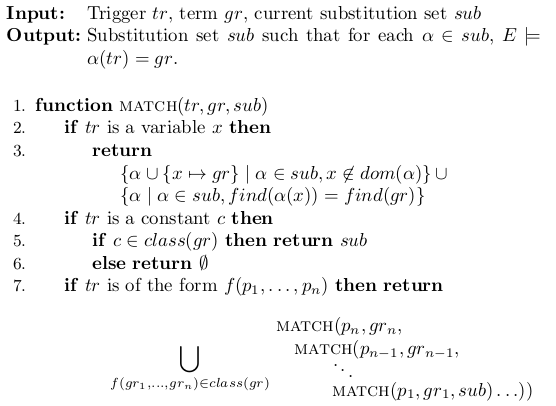
\includegraphics[scale=0.5]{e-matching.png}
\end{frame}

\begin{frame}{E-matching}
$(\forall x.f(x) = x) \wedge (\forall y_1 .\forall y_2 .g(g(y1, y2), y2) = y2) \wedge g(f(g(a, b)), b) \neq b$\newline
\end{frame}

\begin{frame}{E-matching}
$(\forall x.f(x) = x) \wedge (\forall y_1 .\forall y_2 .g(g(y1, y2), y2) = y2) \wedge g(f(g(a, b)), b) \neq b$\newline
match($f(x), f(g(a, b)), \emptyset$)\newline
\end{frame}

\begin{frame}{E-matching}
$(\forall x.f(x) = x) \wedge (\forall y_1 .\forall y_2 .g(g(y1, y2), y2) = y2) \wedge g(f(g(a, b)), b) \neq b$\newline
match($f(x), f(g(a, b)), \emptyset$) =\newline
match($x, g(a, b), \emptyset$)\newline
\end{frame}

\begin{frame}{E-matching}
$(\forall x.f(x) = x) \wedge (\forall y_1 .\forall y_2 .g(g(y1, y2), y2) = y2) \wedge g(f(g(a, b)), b) \neq b$\newline
match($f(x), f(g(a, b)), \emptyset$) =\newline
match($x, g(a, b), \emptyset$) =\newline
$\{x \rightarrow g(a, b)\}$\newline
\end{frame}

\begin{frame}{E-matching}
$(\forall x.f(x) = x) \wedge (\forall y_1 .\forall y_2 .g(g(y1, y2), y2) = y2) \wedge g(f(g(a, b)), b) \neq b$\newline
match($f(x), f(g(a, b), b), \emptyset$) =\newline
match($x, g(a, b), \emptyset$) =\newline
$\{x \rightarrow g(a, b)\}$\newline
$f(g(a, b)) = g(a, b)$
\end{frame}

\begin{frame}{E-matching}
$(\forall x.f(x) = x) \wedge (\forall y_1 .\forall y_2 .g(g(y1, y2), y2) = y2) \wedge g(f(g(a, b)), b) \neq b$\newline
match($g(g(y1, y2), y2), g(f(g(a, b)), b), \emptyset$)
= match($y_2, b, match(g(y_1, y_2 ), f(g(a, b)), \emptyset)$)
= match($y_2, b, match(g(y_1, y_2 ), g(a, b), \emptyset)$)
= match($y_2, b, match(y_2, b, match(y_1 , a, \emptyset))$)
= match($y_2, b, match(y_2, b, \{y_1 \rightarrow a\})$)
= match($y_2, b, \{y_1 \rightarrow a, y_2 \rightarrow b\}$)
= $\{y_1 \rightarrow a, y_2 \rightarrow b\}$\newline
$g(g(a, b), b) = b$\newline
\end{frame}
\begin{frame}{E-matching}
$(\forall x.f(x) = x) \wedge (\forall y_1 .\forall y_2 .g(g(y1, y2), y2) = y2) \wedge g(f(g(a, b)), b) \neq b$\newline
$(f(g(a, b)) = g(a, b)) \wedge (g(g(a, b), b) = b) \wedge (g(f(g(a, b)), b) \neq b)$\newline
\end{frame}

\begin{frame}{E-matching}
$(\forall x.f(2x - x) < x) \wedge (f (a) \ge a)$\newline
\end{frame}

\begin{frame}
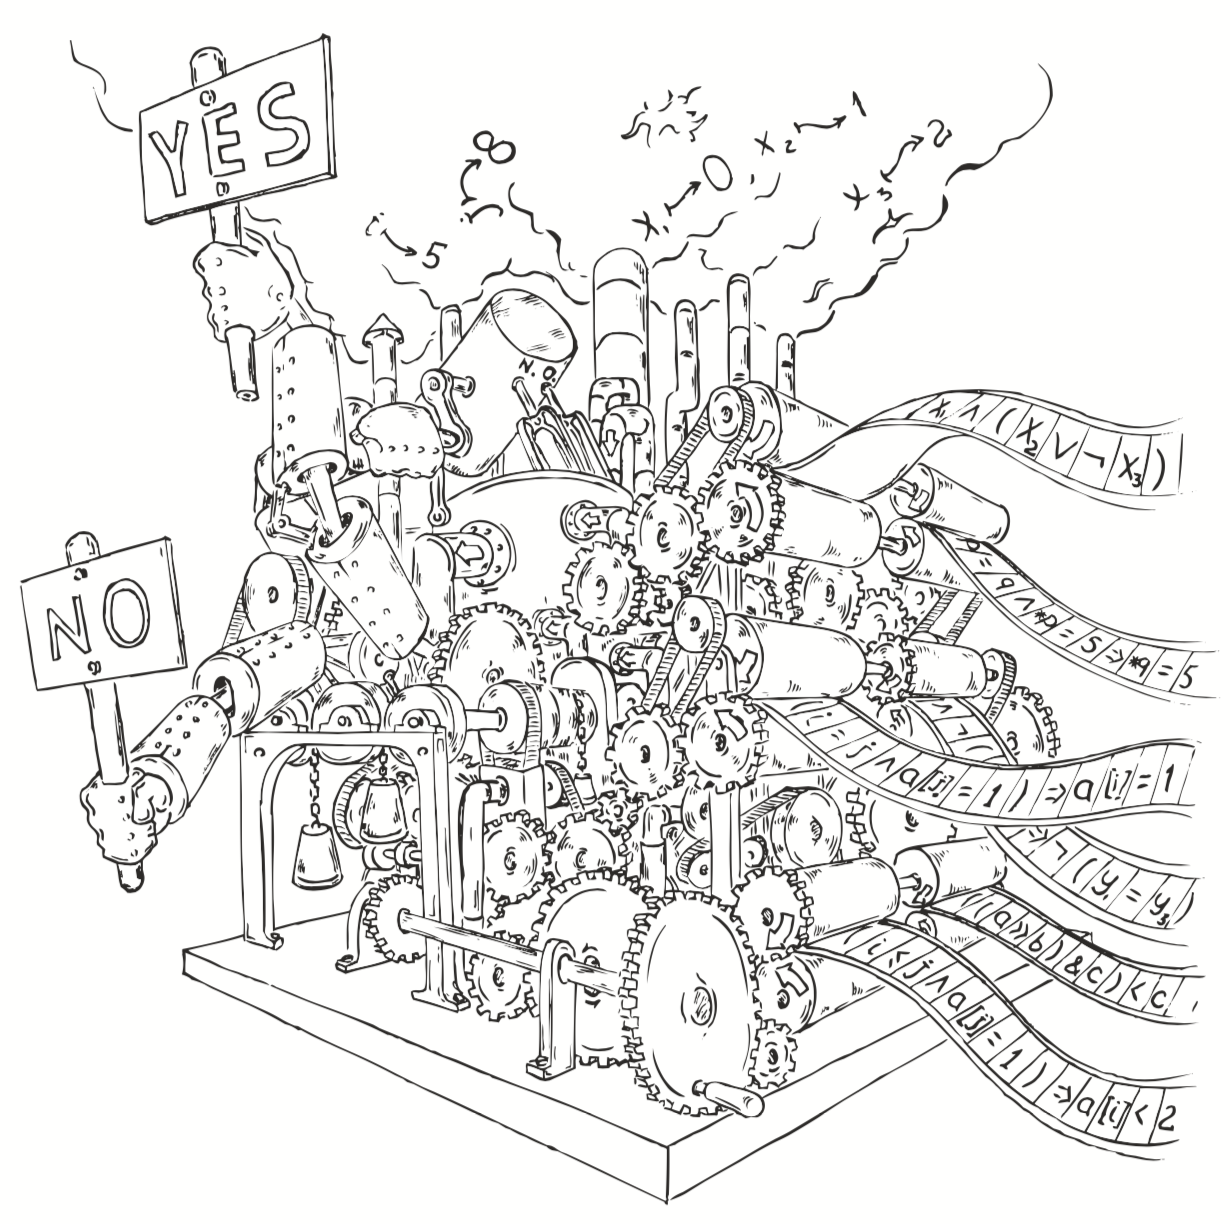
\includegraphics[scale=0.5]{../decision-procedure.png}
\end{frame}

\end{document}
